\section{Product perspective}
\subsection{Scenarios}
\textbf{Company signs up to the platform}\newline
The Company C wants to sign up to the S\&C platform, so a representative R opens the platform and clicks on the "Sign-up" button. The sign-up form is displayed, and R must provide the company's information as well as personal details to be correctly identified as a representative of C. To identify C, R enters the company's name, "C", VAT number, "IT 99999999999", and upload the Certificate of Registration from the Chamber of Commerce. To verify their own identity, R inserts their own company email, "rname.rsurname@companyc.com", and an authorisation letter signed by the CEO of C. 
After a couple of hours, R receives an email with a username for C, "company\_C\_123", and a link to setup a password. R clicks on the link and setup the new password. Now that the password is set, R is be able to log in to the platform, just like other colleagues working at Company C.
\newline\newline
\textbf{Student signs up to the platform and adds their personal information}
\newline
The Student S wants to sign up to the S\&C platform, so opens the platform and clicks on the "Sign-up" button. The sign up form is displayed, and S must provide the academic email, "sname.ssurname@univeristyu.com", and the university name, "University U". S1 is redirected to U's login page, here S1 can login. S1 returns to the S\&C platform Home Page. Now, the student S wants to upload their own personal CV and competences. So, S navigates to their personal page, clicks on "Upload new CV" and uploads the file with the drag and drop function. Then, to insert experiences, skills and attitudes on their profile, S clicks on 
"Add new competence" and fills up the shown form:
\begin{itemize}
    \item New experience:
    \begin{itemize}
        \item Type (Skill, Experience, Attitude): "Skill"
        \item Name: "Coding"
        \item Description (optional): ""
    \end{itemize}
    \item New experience:
    \begin{itemize}
        \item Type (Skill, Experience, Attitude): "Skill"
        \item Name: "Team Working"
        \item Description (optional): ""
    \end{itemize}
    \item New experience:
    \begin{itemize}
        \item Type (Skill, Experience, Attitude): "Attitude"
        \item Name: "Confident"
        \item Description (optional): ""
    \end{itemize}
    \item New experience:
    \begin{itemize}
        \item Type (Skill, Experience, Attitude): "Experience"
        \item Name: "Internship at ABC Company"
        \item Description (optional): ""
    \end{itemize}
\end{itemize}
When finished, S clicks on the "Done" button and is redirected on the profile page where the new competences are shown.
Lastly, S adds a profile picture by clicking on the camera icon and then add a bio by clicking on the pen icon near "Bio".
\newline\newline
\textbf{Company creates an advertisement for an internship position along with the corresponding interview form.}\newline
A representative, R, of a Company C, who is logged in the S\&C platform, wants to create an advertisement for a new internship position available in C. R navigates to the Profile section and clicks on the "Create New Internship Advertisement" button. R is presented with a form where they must provide all relevant details about the internship, so R inserts:
\begin{itemize}
    \item Name of the internship position: "Optimization of delivery transport lines to newsstands"
    \item Location: "Milan"
    \item Candidate's profile: "Management Engineering, Computer Engineering, Mobility Engineering students. Technical skills: data analysis, operational flow analysis, and basic programming with the creation of software for project management. Personal skills: aptitude for working in a Small and Medium-sized Enterprise. Spoken languages: Italian (mandatory) and English"
    \item Project description:
    \begin{itemize}
        \item Educational objectives: "Operation in a multifunctional work environment and ability to analyze and execute a project"
        \item Skills to be acquired: "Fleet analysis, route scheduling, and time slot management"
    \end{itemize}
    \item Terms offered:
    \begin{itemize}
        \item Employment Type: "Full-time (40 hours per week)"
        \item Duration: "4 months"
        \item Total Duration in Hours: "420 hours"
        \item Open Positions: "1"
        \item Travel Requirements: "No"
        \item Benefits: "Networking opportunities within the industry and meal vouchers or subsidized meals"
    \end{itemize}
\end{itemize}
R clicks on the "Done" button, now the new advertisement is published on the platform, and R is redirected to the advertisement page.
R also wants to create the form to be compiled during the interviews for this position. So, R clicks on the button "New Interview Form", and inserts in the presented form all the aspect that are needed to be evaluated during the interview as well as the evaluation methods (e.g., scoring from 1 to 5, written comments):

\begin{itemize}
    \item Name
    \item Surname
    \item Date
    \item Interviewer
    \item General Information (evaluated with "Excellent", "Good", "Satisfactory", "Needs Improvement"):
    \begin{itemize}
        \item Punctuality
        \item Appearance/Professionalism
        \item Communication Skills
    \end{itemize}
    \item Skills and Qualifications:
    \begin{itemize}
        \item Educational Background ("Meets requirements", "Exceeds requirements", "Below requirements")
        \item Relevant Work Experience ("Extensive", "Sufficient", "Limited", "None")
        \item Technical Skills ("Extensive", "Sufficient", "Limited", "None")
        \item Problem-Solving Ability ("Excellent", "Good", "Satisfactory", "Needs Improvement") 
    \end{itemize}
    \item Behavioral Traits (evaluated with "Excellent", "Good", "Satisfactory", "Needs Improvement"):
    \begin{itemize}
        \item Teamwork and Collaboration
        \item Adaptability
        \item Initiative
    \end{itemize}
    \item Job-Specific Questions (evaluated with "Excellent", "Good", "Satisfactory", "Needs Improvement"):
    \begin{itemize}
        \item Knowledge of the Field/Industry
        \item Understanding of the Role
        \item Interest in the Position/Company
    \end{itemize}
    \item Overall Assessment:
    \begin{itemize}
        \item Strengths
        \item Areas for Improvement
        \item Recommendation ("Strongly Recommend", "Recommend", "Recommend with Reservations", "Do Not Recommend")
        \item Additional Comments
    \end{itemize}
\end{itemize}
R clicks on the "Submit" button, so the form is created and available on the ADV page. 
\newline\newline
\textbf{Student looks for an internship and send a request}
\newline
Student S wants to find an internship to enhance their personal career, so, from the homepage, S clicks on the research bar and types the desired characteristics of the internship: "Milan, full-time, paid over 2000€" and presses "Enter". The System shows an alert: there are no results. So, S deletes the characteristics and writes "Milan, full-time". The system shows the correspondent internships, 15 in this case. The student press on the first showed internship in order to visualize the ADV page: it is not in line with S's interests. So, S goes back with the "back arrow" and presses on the second showed internship. S reads the internship's advertise and then clicks on the company's name to visit its page. S approves this internship, so goes back to the internship ADV and presses the "Contact" button to send a request. S add an optional message: "Dear Company C, I am a business management student with a strong interest in marketing strategies, eager to apply my skills and gain hands-on experience. I would be thrilled to contribute to your team as an intern and further develop my expertise. Thank you for considering my application. Best regards, S1."
\newline\newline
\textbf{Student consults a recommendation and send a request}
\newline
Student S wants to check their personal inbox, S notice that they received a recommendation in line with their skills and attitudes. S consults the recommendation about a Company C and clicks on the "Contact" button to send a request, a window opens asking if S wants to add a message, S selects "No". Then S clicks on the Monitor icon and the System shows the monitor view where S can visualize the current state of their request.
\newline\newline
\textbf{Company manages internship requests}\newline
A representative, R, of a Company C, who is logged in the S\&C platform, wants to respond to internship requests received. C navigates to the Inbox Section and opens a message from Student S1. R reads the message and decides to visit S1's personal profile, so R clicks on S1's name and is redirected to their profile. R approves S1 as a potential candidate for the internship, so R clicks on the "Back" button to go back to S1's request and clicks on the "Accept" button. A window opens asking if R also wants to setup a date for the interview. R clicks on the "Setup interview" button and fills out the form with possible date and time slots:
\begin{itemize}
    \item Tuesday, December 10, from 10:00 AM to 11:00 AM or from 11:00 AM to 12:00 PM
    \item Thursday, December 12, from 2:00 PM to 3:00 PM or from 3:00 PM to 4:00 PM
\end{itemize}
When R finishes, they press "Send" and the message is sent to S1. 
R then returns to the Inbox Section and selects another message from Student S2. S2 is not suitable for Company C, so R clicks on the "Reject" button. A windows opens asking if R wants to add a message. R clicks on "Write Message" and writes a few lines to S2 explaining the reasons behind the decision: "Dear S2, thank you for your application for the internship position. After careful consideration, we regret to inform you that we have decided to move forward with other candidates whose qualifications more closely match the requirements for this role. We appreciate the time and effort you invested in your application and encourage you to apply for future opportunities.
Best regards,
R, HR representative", then clicks on "Send".
\newline\newline
\textbf{Student consults an internship request from a Company, consult the offer and the company profile and reject the offer}
\newline
Student S, who is attending an internship at a Company C1, checks their personal inbox and notices that has received a request from a Company C2. S consults the advertise and notice that the proposed internship period is not compatible with the current internship that they are attending. Anyway S decides to have a look of the Company page so press the company name and the System shows the Company Profile. Then S decides that the company is in line with their own interests so goes back to the advertise page clicking the back arrow and presses the "reject" button and writes a short message: "Thank you for the offer, unfortunately, during the period that you proposed I am busy with another company, so I have to reject your propose. However, I really appreciate your company and your work, so do not hesitate to contact me if you have other offers, best wishes, S".
\newline\newline
\textbf{Company writes feedbacks}
\newline
A representative, R, of a Company C, who is logged in the S\&C platform, wants to write some feedback regarding two Students S1 and S2. S1 did an interview for C that went well. However, C decided to go in another direction. R wants to write a positive feedback for S1, so R navigates to the Monitor Section, selects the internship position S1 was applying for, and press the "Feedback" button next to S1's name. R fills out the form presented:
\begin{itemize}
    \item \textbf{Leave an optional comment (it will be displayed on the Student personal page):} "C appreciates your time and preparation for the interview. Although you were not selected, your professionalism and potential stood out. Wishing you success in your future opportunities!"
    \item \textbf{Answer the following questions regarding the student's profile to help make better recommendations} (these answers will only be used by the S\&C system and will not be displayed anywhere):
    \begin{itemize}
        \item \textbf{Are the competences displayed on the student's profile consistent with their actual abilities?} (Yes, No, Not checked):
        \begin{itemize}
            \item Coding skills: "Yes"
            \item English C1: "Not checked"
            \item Effective communication: "Yes"
            \item Proactive Mindset: "Not checked"
            \item Team-Oriented: "Not checked"
        \end{itemize}
        \item \textbf{Is the CV consistent with the student's actual experiences?}: "No"
        \item Please explain why the CV is not consistent: "The student did not work part-time at Company ABC in Milan"
    \end{itemize}
    \item\textbf{Answer the following questions regarding the impression received during the interview with a number between 1 (Needs Improvement) to 4 (Accomplished)}:
    \begin{itemize}
        \item Punctuality 
        \item Communication Skills
        \item Critical Thinking Skills
        \item Confidence and Poise
        \item Knowledge of the Company
        \item Enthusiasm for the Role
    \end{itemize}
\end{itemize}

R writes the comment about S1 and presses "Submit". The comment will appear on S1's personal page.
On the other hand, Student S2 did a brief internship, but C is not satisfied with S2's behavior. To write feedback about S2, R navigates to the Monitoring Section and then to the Students Employed section, clicks on S2's name, and select "Feedback".  R fills out the form presented:
\begin{itemize}
    \item \textbf{Leave an optional comment (it will be displayed on the Student personal page):} "We had the opportunity to host S2 for a brief internship at C. During this time, we observed some challenges in punctuality, as consistent tardiness impacted daily productivity. Additionally, while S2 presented a skill set on their CV, these skills did not align with the expectations required for the role. We encourage S2 to focus on enhancing time management and further developing the skills highlighted in their resume to meet the demands of future opportunities. We believe in the potential for growth and improvement through constructive feedback and continued effort. Best wishes for future endeavors."
    \item \textbf{Answer the following questions regarding the student's profile to help make better recommendations} (these answers will only be used by the S\&C system and will not be displayed anywhere):
    \begin{itemize}
        \item \textbf{Are the competences displayed on the student's profile consistent with their actual abilities?} (Yes, No, Not checked):
        \begin{itemize}
            \item Data analysis and visualization: "No"
            \item Project management tools : "Yes"
            \item Time management: "No"
            \item Adaptability: "Yes"
        \end{itemize}
        \item \textbf{Is the CV consistent with the student's actual experiences?}: "No"
        \item Please explain why the CV is not consistent: "Competences described above."
    \end{itemize}
    \item\textbf{Answer the following questions regarding the impression received during the internship with a number between 1 (Needs Improvement) to 4 (Accomplished)}:
    \begin{itemize}
        \item Punctuality 
        \item Communication Skills
        \item Critical Thinking Skills
        \item Confidence and Poise
        \item Ability to Handle Stress
        \item Team Collaboration 
        \item Enthusiasm for the Role
    \end{itemize}
\end{itemize}
The comment will appear on S2's personal page.

\subsection{Domain Class Diagram}
\begin{figure}[H]
    \centering
    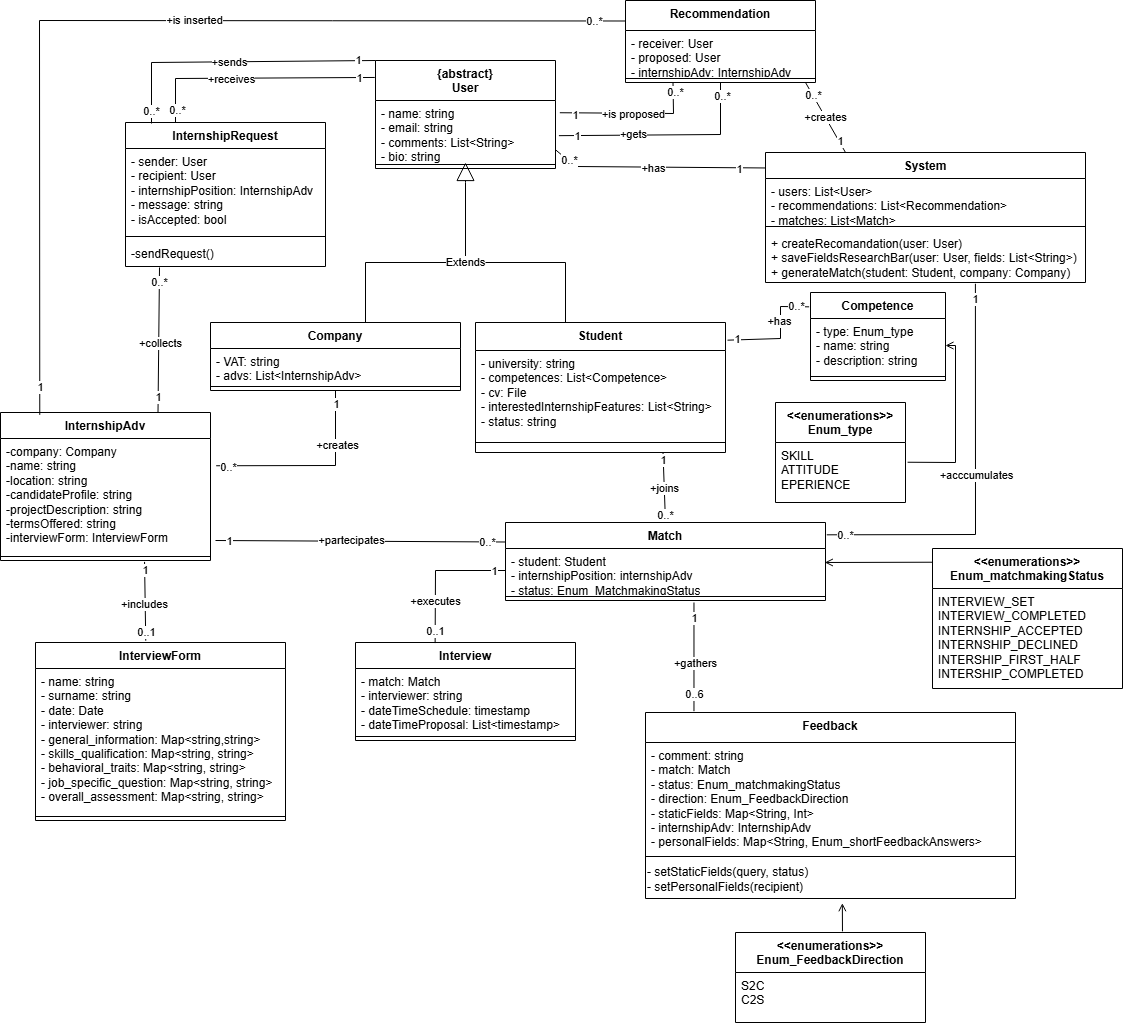
\includegraphics[width=15cm]{Images/RASD-Domain Class Diagram.drawio.png}
    \caption{UML Domain Class Diagram}
\end{figure}
This Domain Class Diagram shows all the classes that will be created to manage the system and the relations between them. Only the relevant methods are present.
Here follows a more detailed explanation of the classes and the relations.\newline
The class \textbf{System} manages the users, creates the recommendations (represented by the class \textbf{Recommendation}), and handles the matches between students and internship positions. The abstract class \textbf{User} is created to generalise the two types of user that navigate through the system: Student and Company. \textbf{Student} is the class dedicated to university students, in particular, it has a list of \textbf{Competence}s, each one of them can be one of three types (\textbf{Skill}, \textbf{Attitude}, \textbf{Experience}) and has a description. The list called \textbf{interestedIntenshipFeatures} contains the fileds inserted in the search bar by the student, they are used by the System to create appropriate recommendations. \textbf{Company} handles the profile of a company, it is linked to the \textbf{InternshipAdv} class that manages the internship advertisements. This class contains all the relevant information that will be shown in the ADV, in particular it contains the field \textbf{candidateProfile} that will be used by the System to make consistent recommendation. It also includes the \textbf{InterviewForm} that contains all the information that has to be inserted in the form to be used during the interview for the advertised internship position. It can be inserted after a while from the creation of the ADV, so, for this reason, the cardinality is 0 to 1.\newline
The class \textbf{InternshipRequest} represent the request sent by the company (or the student) to the student (or the company) regarding a specific internship ADV. The boolean \textbf{isAccepted} will turn true if the counterpart accepts the propose. \newline
When a contact is made then a match between the student and the ADV is created. This is handeld by the class \textbf{Match} with the field \textbf{matchmakingStatus} that keeps track of the status of the match, it goes from the setting of the interview to the completion of the internship. It has a relation ("executes") with the class \textbf{Interview} that contains the information relevant for the interview between that specific Match. The class Match is also related to the class \textbf{Feedback}. A feedback can be created only in specific states of the match: after the interview is terminated ({INTERVIEW\_COMPLETED}), at the first half of the internship ({INTERNSHIP\_FIRST\_HALF}) and at the end ({INTERNSHIP\_COMPLETED}). Drafting the feedback is optional, and can be done in both directions: by the student for the company (S2C) and by the company for the student (C2S). This explains the cardinality 0 (it is optional) to 6 both the student and the company answer to all the feedback of the three states). 

\subsection{State Diagrams}
\textbf{Sign up and Login}\newline
\begin{figure}[H]
    \centering
    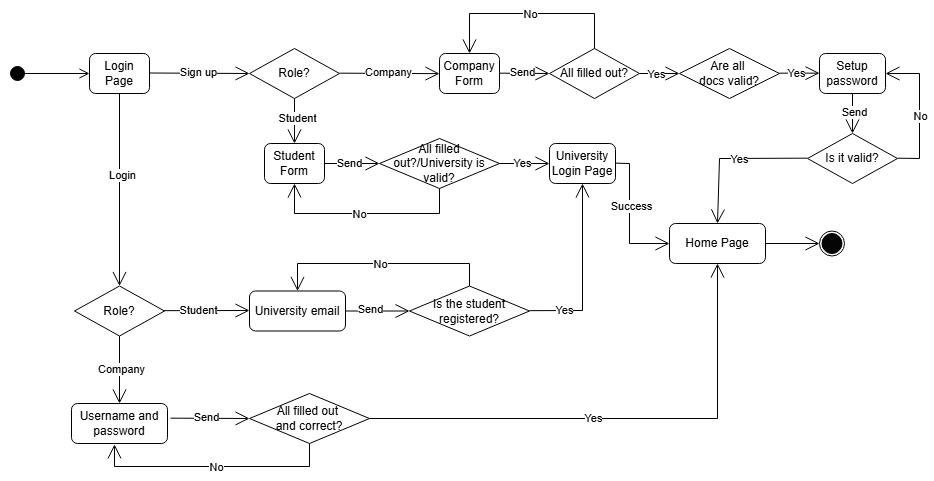
\includegraphics[width=15cm]{Images/State_Diagrams/RASD-SD-login_signup.drawio.png}
    \caption{Sign up and Login State Diagram}
\end{figure}
This State Diagram describes the processes of Sign Up and Login for both Companies and Students. 
\newline

\textbf{Update Student's Profile}\newline
\begin{figure}[H]
    \centering
    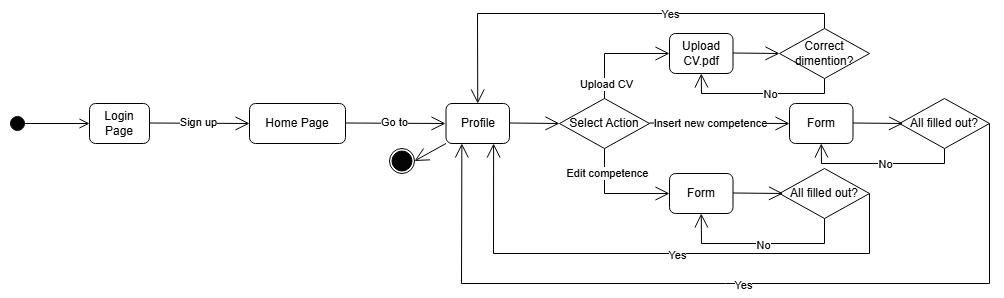
\includegraphics[width=15cm]{Images/State_Diagrams/RASD-SD-Update student profile.drawio.png}
    \caption{Update Student's Profile State Diagram}
\end{figure}
This diagram illustrates how a Student can updates their profile. The Login step is implicit because it is shown in the first diagram. The Student can upload a new CV, insert new competences, or edit the ones already present. 
\newline

\textbf{Creation of an Internship Advertisement}\newline
\begin{figure}[H]
    \centering
    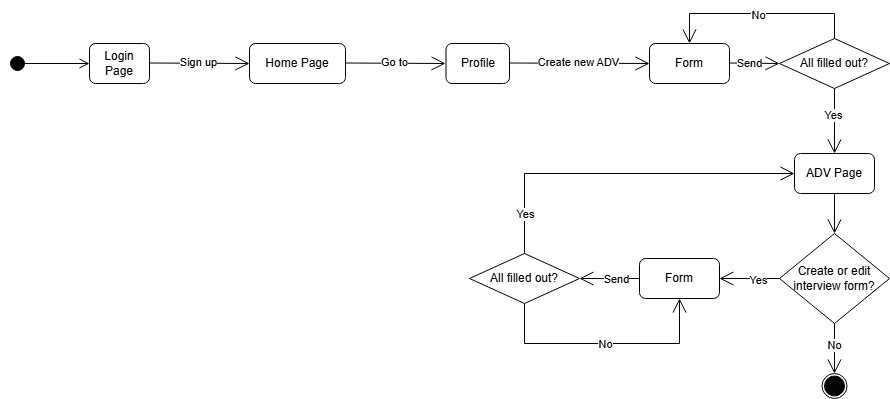
\includegraphics[width=15cm]{Images/State_Diagrams/RASD-SD-create adv.drawio.png}
    \caption{Creation of an Internship Advertisement State Diagram}
\end{figure}
This graph shows the process of the creation of an Internship Advertisement done by a Company. As before, the Login step is implicit. The Company can also decide whether to create the Interview Form immediately.
\newline

\textbf{Company's Matchmaking Process}\newline
\begin{figure}[H]
    \centering
    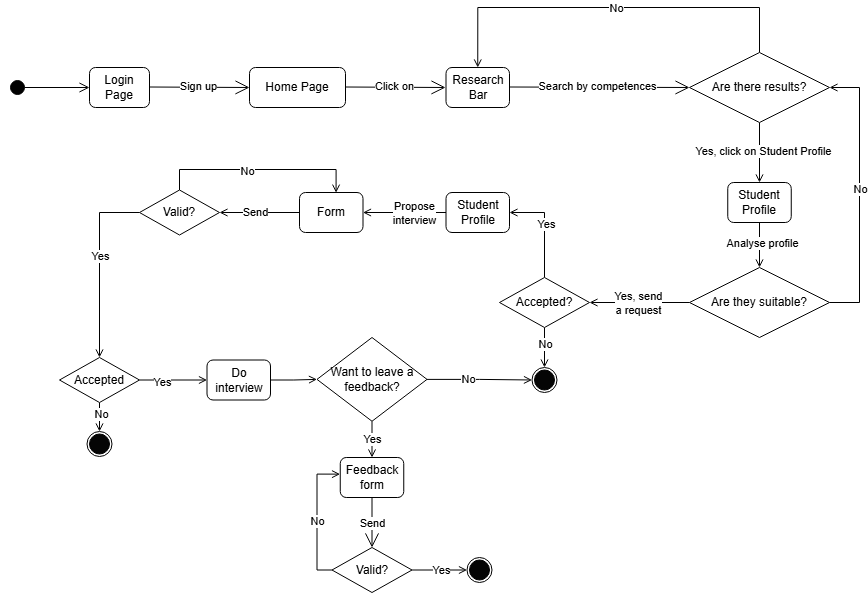
\includegraphics[width=15cm]{Images/State_Diagrams/RASD-SD-Matchmaking.drawio.png}
    \caption{Company's Matchmaking Process State Diagram}
\end{figure}
This State Diagram describes the process that a Company has to go through in order to search for a candidate, contact them and set up an interview. The Login step is implicit.
\newline

\textbf{Feedback}\newline
\begin{figure}[H]
    \centering
    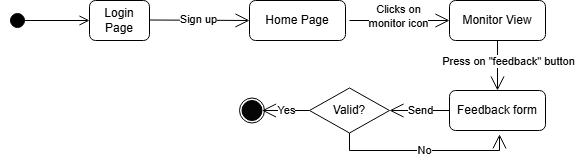
\includegraphics[width=15cm]{Images/State_Diagrams/RASD-SD-Feedback.drawio.png}
    \caption{Feedback State Diagram}
\end{figure}
This State Diagram shows how a User can leave a feedback. The Login step is implicit and it is assumed that the user has matches.
\newline

\section{Product functions}
\textbf{Sign up and Login}\newline
The S\&C platform allows users to register and log in depending on their role. Students can manage both the sign up and log in through their university credentials, i.e. the system redirects them to their university's website. A representative of a Company can register it by filling a form where they have to identify both the company and themselves. To identify the Company, they have to insert the VAT number and upload a certificate of registration at the Chamber of Commerce. To identify themselves, they have to insert their own company email and upload a letter of authorisation or official assignment signed by the CEO or an HR referent. The uploaded documentation will be reviewed by S\&C employees and if everything is correct, an email will be sent to the representative containing a username and a link to set a password.

\textbf{Update Student's profile}\newline
Students can update their profile in many ways: they can upload their CV (as a pdf) for the first time, but also upload a new version if they have updated it. They can also insert personal competences (such as skills, experiences, and attitudes) to be shown in their profile. Such competences can be modified and/or deleted whenever they want.

\textbf{Create internship's advertise}\newline
The platform allows representatives of Companies to create internship advertises where they can specify the project of the internship, the profile of the candidate they are looking for, and the terms offered. These advs can be modified or deleted from the platform.

\textbf{Proactive Research}\newline
The platform allows users to use a search bar. Students can find internships by inserting specific requirements about the project and/or the teams offered. If the system finds some suitable internships, it shows them to the Student who can click on them to visualise the adv and/on the Company's profile and eventually contact them. Companies' representatives can search for suitable candidates through this search bar by inserting the competences they are looking for. If the system finds Some suitable candidates, it shows them to the representative who can click on them to visualise the Student's profile and eventually contact them. 

\textbf{Recommendation}\newline
S\&C notifies users about potential matches. Proactive research criteria provided by students are used to recommend suitable internship opportunities. Similarly, the candidate profile specified in an internship advertisement is used to recommend matching students to companies. Recommendations are also based on the feedbacks received by the users. These recommendations are shared with the users and can be accessed via the Inbox section present in their profile. From the recommendation notifications, students can explore the internship advertisement and the company's profile, while companies can view the students' profiles.

\textbf{Matching between company and student and establishment of a contact}\newline
S\&C allows Student to contact Company that find on the platform through the research bar or thanks to the recommendation. S\&C also allows Company to contact Student that they found by the research bar or thanks to the recommendation. The system also will inform the Students and Companies if someone wants to contact them, the user contacted will see a message in the inbox section, and thorough that they will be able to get information about the user who contacted them. When receiving a message, the user can decide to reject the offer or to establish a contact.

\textbf{Selection process}\newline
S\&C allows Company, after they establish a contact with a student, to propose to the student some Date and Time slots in order to schedule an interview, the student will be pale to accept one of the proposals or reject them all. The system will provider assistance to Company during the interview too, indeed S\&C allows Company to create a standard form where they can write all the aspects that the interviewer will evaluate during the meeting.

\textbf{Feedback}\newline
S\&C allows Students to leave a feedback about the Company or some aspect of a Company during the selection period or about the internship that they are attending or have just finished. And allows Company to write feedback about a Student after the review, during the internship, or when the internship is just finished. The platform will use this feedback to enhance its recommendation system.

\textbf{Monitoring of the matchmaking process}\newline
S\&C allows every user to monitor their situation, in particular help to understand in which state of matchmaking or internship the users are. For Company S\&C allows to monitor the state of every student that is in contact with and with the ones who are attending an internship in the company, allowing us to leave a feedback to them. For Student allows to monitor the state of the matchmaking with the companies or the state of the internship that their are attending.

\section{User Characteristics}. Users who can interact with the system can be subdivided into two groups:
\begin{enumerate}
    \item University students seeking an internship related to their field of study. 
    \item Companies looking for university students with specific qualifications to fill internship positions.
\end{enumerate}



\section{Assumption, dependencies, and constraints}
\begin{itemize}
    \item[\text{[D1]}] Companies offer real internship positions.
    \item[\text{[D2]}] Students search for internship related to their course.
    \item[\text{[D3]}] Students write their own CV according to their real experiences, skills, and attitudes.
    \item[\text{[D4]}] The experiences, skills, and attitudes shown in the students' profiles are consistent with those in their respective CVs.
    \item[\text{[D5]}] Companies are honest in listing the projects and the terms offered.
    \item[\text{[D6]}] Students and companies are honest when giving feedbacks.
    \item[\text{[D7]}] Students and companies have access to a working Internet connection.
    \item[\text{[D8]}] Employees of the S\&C platform that checks the validity of a Company are capable and honest.
\end{itemize}